\documentclass[a4paper]{report}

\usepackage[
    left    = 15mm,
    right   = 15mm,
    top     = 15mm,
    bottom  = 15mm,
]{geometry}

\usepackage{siunitx}
\usepackage{xcolor}
\usepackage{tcolorbox}
\usepackage{booktabs}
\usepackage{titletoc}
\usepackage{enumitem}
\usepackage{tabularx, tabu, ragged2e}
\usepackage[MnSymbol]{mathspec}

\setcounter{secnumdepth}{0}

\setallmainfonts{Minion Pro}

\pagestyle{empty}
\renewcommand{\arraystretch}{1.5}
\linespread{1.3}
\aboverulesep=1.6ex
\belowrulesep=1.6ex

\setlist[description]{
    font=\Large,
    style=multiline,
    leftmargin=20mm,
}

\begin{document}
    \begin{minipage}{\textwidth}
        \begin{minipage}{0.2\textwidth}
            
\includegraphics[width=32mm]{input/logo.jpg}
        \end{minipage}
        \begin{minipage}{0.58\textwidth}
            \centering
            \fontsize{40}{50}\selectfont
            Astroworkshop\\
            \large
            of the Comenius University\\
            2020
        \end{minipage}
        \begin{minipage}{0.2\textwidth}
            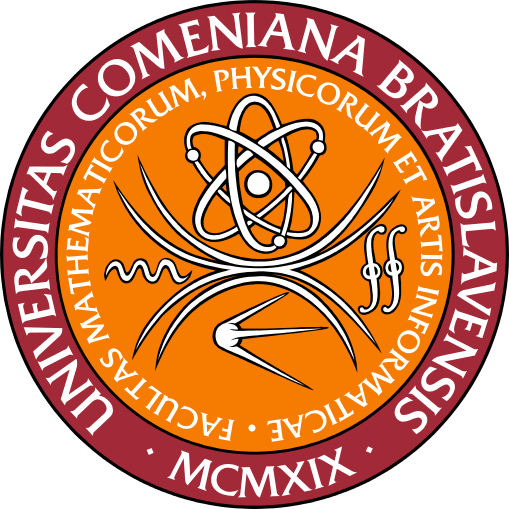
\includegraphics[width=32mm]{input/fmfi.png}
        \end{minipage}
    \end{minipage}
    \vspace*{10mm}

    \begin{tabularx}{\textwidth}{>{}p{2cm} >{\RaggedRight}X}
        \textbf{Miesto}:    & AGO Modra \\
        \textbf{Dátum}:     & 2020-03-05 -- 2020-03-08 \\
        \textbf{Organizátori}: &
            Martin Baláž,             Patrik Čechvala,             Karol Havrila,             Emil Puha,             Matej Zigo             \\
    \end{tabularx}

            \section{\color[rgb]{0, 0.1, 0.4}{štvrtok}}

        \begin{tabularx}{\textwidth}{>{}p{2cm} >{\RaggedRight}X}
            \toprule
                            {\Large 19:00} & {\Large Otvorenie 7. ročníka ASTRO workshopu} \\
                                                                                                        \bottomrule
        \end{tabularx}

        \begin{description}
                            \item[19:00]
                    {\Large Otvorenie 7. ročníka ASTRO workshopu} \\[1ex]
                                                                                
                    \end{description}


                                    \begin{tcolorbox}
                            \subsection{19:00 \hfill Otvorenie 7. ročníka ASTRO workshopu}
                                                            \end{tcolorbox}
                                \section{\color[rgb]{0, 0.1, 0.4}{piatok}}

        \begin{tabularx}{\textwidth}{>{}p{2cm} >{\RaggedRight}X}
            \toprule
                            {\Large 09:00} & {\Large Spoločné raňajky} \\
                                                                                \midrule                            {\Large 10:00} & {\Large Expedícia Hawaii 2020} \\
                                            & \textit{\textbf{Juraj Tóth}} \\
                                                                & \textit{FMFI UK} \\
                                                            \midrule                            {\Large 10:30} & {\Large Kerbal Space Program} \\
                                            & \textit{\textbf{Martin Baláž}} \\
                                                                & \textit{FMFI UK} \\
                                                                & Kerbal Space Program is one of the most successful realistic space program simulation games. Apart from entertainment, it is very useful in teaching and intuitively understanding basic concepts of orbital mechanics, rocket construction and space mission design.
 \\
                                        \midrule                            {\Large 11:00} & {\Large Dojmy z konferencie AstroEdu v Garchingu} \\
                                            & \textit{\textbf{Patrik Čechvala}} \\
                                                                                    & 16.--18. septembra 2019 sa konala v Garchingu pri Mníchove konferencia zameraná na vyučovanie a popularizáciu astronómie organizovaná Medzinárodnou astronomickou úniou IAU. Konferencia sa odohrávala v návštevníckom centre Európskeho južného observatória ESO Supernova. Na tejto konferencii sme prezentovali príspevok, ktorý vznikol v spolupráci s doktorandkami z Katedry didaktiky. Ukážeme si niektoré zaujímavosti z tejto konferencie. Špeciálne sa budeme venovať samotnému návšteníckemu centru ESO Supernova, ktoré pozostáva z planetária a výstavných plôch.
 \\
                                        \midrule                            {\Large 12:00} & {\Large Structure of the outer Galactic disk} \\
                                            & \textit{\textbf{Žofia Chrobáková}} \\
                                                                & \textit{Instituto de Astrofisica Canarías} \\
                                                                & The structure of the outer disk of our Galaxy is still not well described and there are many features that need to be better understood. Gaia DR2 provides data in unprecedented quality that can be analyzed to shed some light on the outermost parts of the Milky Way. We calculated stellar density using star counts obtained from Gaia DR2, up to galactocentric distance $R$ = 20 kpc using a deconvolution technique in the parallax errors. To recover star counts, we carry out the deconvolution, using the Lucy's inversion method of the Fredholm integral equations of the first kind, without assuming any prior. We analyzed the density in order to study the structure of the outer Galactic disk and created density maps, where we can see structural features, mainly the warp. We studied the warp in greater detail, fitting it with multiple models and analyzing its properties. When we study the northern and the southern warps separately, we get an asymmetry of \textasciitilde\SI{25}{\percent} larger amplitude in the north. We also study the flare -- the increase of the scale-height with galactocentric distance. We will show preliminary results of our analysis, which shed some light on possibility of flaring of the Galactic disk in the remote regions of the Galaxy.
 \\
                                        \midrule                            {\Large 13:00} & {\Large Prvý hnedý trpaslík z vesmírnej misie TESS objavený v Ondřejove} \\
                                            & \textit{\textbf{Ján Šubjak}} \\
                                                                & \textit{Astronomický ústav AV ČR Ondřejov} \\
                                                                & V súčasnosti sú známe približne dve desiatky tranzitujúcich hnedých trpaslíkov s presne zmeranou hmotnosťou a polomerom. K nim sa nedávno pridal systém TOI-503 a pár ďalších čerstvo objavených systémov z vesmírnej misie TESS a potvrdených dodatočnou spektroskopiou. Napriek úspechom tejto misie však ostávame limitovaný pri štúdiu a pochopení populácie hnedých trpaslíkov vzhľadom na malý počet jej objavených členov a každý nový člen sa stáva testom pre súčasné modely a poznatky. TOI-503 je prvý hnedý trpaslík z vesmírnej misie TESS a vôbec prvý v okolí hviezdy spektrálneho typu Am. Podrobne sme analyzovali získané fotometrické a spektroskopické dáta pre tento systém a charakterizovali jeho parametre, ako aj možné spôsoby formovania.
 \\
                                        \midrule                            {\Large 14:00} & {\Large Optimisation of double-station balloon flights for meteor observation: Prediction of the MALBEC nacelle trajectory} \\
                                            & \textit{\textbf{Danica Žilková}} \\
                                                                & \textit{FMFI UK} \\
                                                                & The “Meteor Automated Light Balloon Experimental Camera” (MALBEC) project aims at the observation of meteors from stratospheric altitude. The advantage is mainly to guarantee the success of an observation run of a meteor shower, even in presence of clouds. In order to fully exploit the scientific potential of a meteor observation (e.g. derive the internal structure and origin via the measure of tensile strength and orbit), double-station setup is required. The consequence for MALBEC is the necessity of stabilisation and we show that a 3-axis stabilisation is necessary. In addition, the two stations must be separated by a distance ranging from \textasciitilde\SIrange{40}{110}{\kilo\metre}, and the cameras must point towards the same portion of atmosphere. We show that under usual circumstances, double station stratospheric observation is possible since the distance and the azimuth between the two balloons (experiencing different atmospheric conditions) varies in small proportions. Under usual slow wind conditions, the distance between the stations varies by a few km and the elevation of the azimuth and elevation of the cameras needed to observe the same portion of atmosphere varies by a few deg only. In order to demonstrate the feasibility of stratospheric double station meteor observation we developed a tool to simulate the flight and predict the trajectory of the MALBEC nacelle. This will be further illustrated in the upcoming presentation.
 \\
                                                                \bottomrule
        \end{tabularx}

        \begin{description}
                            \item[09:00]
                    {\Large Spoločné raňajky} \\[1ex]
                                                                                \rule{\paperwidth}{0.4pt}
                            \item[10:00]
                    {\Large Expedícia Hawaii 2020} \\[1ex]
                                            \textit{\textbf{Juraj Tóth}} \\%
                                        \textit{FMFI UK} \\[1ex]                                        \rule{\paperwidth}{0.4pt}
                            \item[10:30]
                    {\Large Kerbal Space Program} \\[1ex]
                                            \textit{\textbf{Martin Baláž}} \\%
                                        \textit{FMFI UK} \\[1ex]                    Kerbal Space Program is one of the most successful realistic space program simulation games. Apart from entertainment, it is very useful in teaching and intuitively understanding basic concepts of orbital mechanics, rocket construction and space mission design.
 \\                    \rule{\paperwidth}{0.4pt}
                            \item[11:00]
                    {\Large Dojmy z konferencie AstroEdu v Garchingu} \\[1ex]
                                            \textit{\textbf{Patrik Čechvala}} \\%
                                                            16.--18. septembra 2019 sa konala v Garchingu pri Mníchove konferencia zameraná na vyučovanie a popularizáciu astronómie organizovaná Medzinárodnou astronomickou úniou IAU. Konferencia sa odohrávala v návštevníckom centre Európskeho južného observatória ESO Supernova. Na tejto konferencii sme prezentovali príspevok, ktorý vznikol v spolupráci s doktorandkami z Katedry didaktiky. Ukážeme si niektoré zaujímavosti z tejto konferencie. Špeciálne sa budeme venovať samotnému návšteníckemu centru ESO Supernova, ktoré pozostáva z planetária a výstavných plôch.
 \\                    \rule{\paperwidth}{0.4pt}
                            \item[12:00]
                    {\Large Structure of the outer Galactic disk} \\[1ex]
                                            \textit{\textbf{Žofia Chrobáková}} \\%
                                        \textit{Instituto de Astrofisica Canarías} \\[1ex]                    The structure of the outer disk of our Galaxy is still not well described and there are many features that need to be better understood. Gaia DR2 provides data in unprecedented quality that can be analyzed to shed some light on the outermost parts of the Milky Way. We calculated stellar density using star counts obtained from Gaia DR2, up to galactocentric distance $R$ = 20 kpc using a deconvolution technique in the parallax errors. To recover star counts, we carry out the deconvolution, using the Lucy's inversion method of the Fredholm integral equations of the first kind, without assuming any prior. We analyzed the density in order to study the structure of the outer Galactic disk and created density maps, where we can see structural features, mainly the warp. We studied the warp in greater detail, fitting it with multiple models and analyzing its properties. When we study the northern and the southern warps separately, we get an asymmetry of \textasciitilde\SI{25}{\percent} larger amplitude in the north. We also study the flare -- the increase of the scale-height with galactocentric distance. We will show preliminary results of our analysis, which shed some light on possibility of flaring of the Galactic disk in the remote regions of the Galaxy.
 \\                    \rule{\paperwidth}{0.4pt}
                            \item[13:00]
                    {\Large Prvý hnedý trpaslík z vesmírnej misie TESS objavený v Ondřejove} \\[1ex]
                                            \textit{\textbf{Ján Šubjak}} \\%
                                        \textit{Astronomický ústav AV ČR Ondřejov} \\[1ex]                    V súčasnosti sú známe približne dve desiatky tranzitujúcich hnedých trpaslíkov s presne zmeranou hmotnosťou a polomerom. K nim sa nedávno pridal systém TOI-503 a pár ďalších čerstvo objavených systémov z vesmírnej misie TESS a potvrdených dodatočnou spektroskopiou. Napriek úspechom tejto misie však ostávame limitovaný pri štúdiu a pochopení populácie hnedých trpaslíkov vzhľadom na malý počet jej objavených členov a každý nový člen sa stáva testom pre súčasné modely a poznatky. TOI-503 je prvý hnedý trpaslík z vesmírnej misie TESS a vôbec prvý v okolí hviezdy spektrálneho typu Am. Podrobne sme analyzovali získané fotometrické a spektroskopické dáta pre tento systém a charakterizovali jeho parametre, ako aj možné spôsoby formovania.
 \\                    \rule{\paperwidth}{0.4pt}
                            \item[14:00]
                    {\Large Optimisation of double-station balloon flights for meteor observation: Prediction of the MALBEC nacelle trajectory} \\[1ex]
                                            \textit{\textbf{Danica Žilková}} \\%
                                        \textit{FMFI UK} \\[1ex]                    The “Meteor Automated Light Balloon Experimental Camera” (MALBEC) project aims at the observation of meteors from stratospheric altitude. The advantage is mainly to guarantee the success of an observation run of a meteor shower, even in presence of clouds. In order to fully exploit the scientific potential of a meteor observation (e.g. derive the internal structure and origin via the measure of tensile strength and orbit), double-station setup is required. The consequence for MALBEC is the necessity of stabilisation and we show that a 3-axis stabilisation is necessary. In addition, the two stations must be separated by a distance ranging from \textasciitilde\SIrange{40}{110}{\kilo\metre}, and the cameras must point towards the same portion of atmosphere. We show that under usual circumstances, double station stratospheric observation is possible since the distance and the azimuth between the two balloons (experiencing different atmospheric conditions) varies in small proportions. Under usual slow wind conditions, the distance between the stations varies by a few km and the elevation of the azimuth and elevation of the cameras needed to observe the same portion of atmosphere varies by a few deg only. In order to demonstrate the feasibility of stratospheric double station meteor observation we developed a tool to simulate the flight and predict the trajectory of the MALBEC nacelle. This will be further illustrated in the upcoming presentation.
 \\                    
                    \end{description}


                                    \begin{tcolorbox}
                            \subsection{09:00 \hfill Spoločné raňajky}
                                                            \end{tcolorbox}
                                                \begin{tcolorbox}
                            \subsection{10:00 \hfill Expedícia Hawaii 2020}
                                    \hfill \textit{Juraj Tóth} \\
                                                            \end{tcolorbox}
                                                \begin{tcolorbox}
                            \subsection{10:30 \hfill Kerbal Space Program}
                                    \hfill \textit{Martin Baláž} \\
                                                    Kerbal Space Program is one of the most successful realistic space program simulation games. Apart from entertainment, it is very useful in teaching and intuitively understanding basic concepts of orbital mechanics, rocket construction and space mission design.

                                            \end{tcolorbox}
                                                \begin{tcolorbox}
                            \subsection{11:00 \hfill Dojmy z konferencie AstroEdu v Garchingu}
                                    \hfill \textit{Patrik Čechvala} \\
                                                    16.--18. septembra 2019 sa konala v Garchingu pri Mníchove konferencia zameraná na vyučovanie a popularizáciu astronómie organizovaná Medzinárodnou astronomickou úniou IAU. Konferencia sa odohrávala v návštevníckom centre Európskeho južného observatória ESO Supernova. Na tejto konferencii sme prezentovali príspevok, ktorý vznikol v spolupráci s doktorandkami z Katedry didaktiky. Ukážeme si niektoré zaujímavosti z tejto konferencie. Špeciálne sa budeme venovať samotnému návšteníckemu centru ESO Supernova, ktoré pozostáva z planetária a výstavných plôch.

                                            \end{tcolorbox}
                                                \begin{tcolorbox}
                            \subsection{12:00 \hfill Structure of the outer Galactic disk}
                                    \hfill \textit{Žofia Chrobáková} \\
                                                    The structure of the outer disk of our Galaxy is still not well described and there are many features that need to be better understood. Gaia DR2 provides data in unprecedented quality that can be analyzed to shed some light on the outermost parts of the Milky Way. We calculated stellar density using star counts obtained from Gaia DR2, up to galactocentric distance $R$ = 20 kpc using a deconvolution technique in the parallax errors. To recover star counts, we carry out the deconvolution, using the Lucy's inversion method of the Fredholm integral equations of the first kind, without assuming any prior. We analyzed the density in order to study the structure of the outer Galactic disk and created density maps, where we can see structural features, mainly the warp. We studied the warp in greater detail, fitting it with multiple models and analyzing its properties. When we study the northern and the southern warps separately, we get an asymmetry of \textasciitilde\SI{25}{\percent} larger amplitude in the north. We also study the flare -- the increase of the scale-height with galactocentric distance. We will show preliminary results of our analysis, which shed some light on possibility of flaring of the Galactic disk in the remote regions of the Galaxy.

                                            \end{tcolorbox}
                                                \begin{tcolorbox}
                            \subsection{13:00 \hfill Prvý hnedý trpaslík z vesmírnej misie TESS objavený v Ondřejove}
                                    \hfill \textit{Ján Šubjak} \\
                                                    V súčasnosti sú známe približne dve desiatky tranzitujúcich hnedých trpaslíkov s presne zmeranou hmotnosťou a polomerom. K nim sa nedávno pridal systém TOI-503 a pár ďalších čerstvo objavených systémov z vesmírnej misie TESS a potvrdených dodatočnou spektroskopiou. Napriek úspechom tejto misie však ostávame limitovaný pri štúdiu a pochopení populácie hnedých trpaslíkov vzhľadom na malý počet jej objavených členov a každý nový člen sa stáva testom pre súčasné modely a poznatky. TOI-503 je prvý hnedý trpaslík z vesmírnej misie TESS a vôbec prvý v okolí hviezdy spektrálneho typu Am. Podrobne sme analyzovali získané fotometrické a spektroskopické dáta pre tento systém a charakterizovali jeho parametre, ako aj možné spôsoby formovania.

                                            \end{tcolorbox}
                                                \begin{tcolorbox}
                            \subsection{14:00 \hfill Optimisation of double-station balloon flights for meteor observation: Prediction of the MALBEC nacelle trajectory}
                                    \hfill \textit{Danica Žilková} \\
                                                    The “Meteor Automated Light Balloon Experimental Camera” (MALBEC) project aims at the observation of meteors from stratospheric altitude. The advantage is mainly to guarantee the success of an observation run of a meteor shower, even in presence of clouds. In order to fully exploit the scientific potential of a meteor observation (e.g. derive the internal structure and origin via the measure of tensile strength and orbit), double-station setup is required. The consequence for MALBEC is the necessity of stabilisation and we show that a 3-axis stabilisation is necessary. In addition, the two stations must be separated by a distance ranging from \textasciitilde\SIrange{40}{110}{\kilo\metre}, and the cameras must point towards the same portion of atmosphere. We show that under usual circumstances, double station stratospheric observation is possible since the distance and the azimuth between the two balloons (experiencing different atmospheric conditions) varies in small proportions. Under usual slow wind conditions, the distance between the stations varies by a few km and the elevation of the azimuth and elevation of the cameras needed to observe the same portion of atmosphere varies by a few deg only. In order to demonstrate the feasibility of stratospheric double station meteor observation we developed a tool to simulate the flight and predict the trajectory of the MALBEC nacelle. This will be further illustrated in the upcoming presentation.

                                            \end{tcolorbox}
                                \section{\color[rgb]{0, 0.1, 0.4}{sobota}}

        \begin{tabularx}{\textwidth}{>{}p{2cm} >{\RaggedRight}X}
            \toprule
                            {\Large 14:00} & {\Large Optimisation of double-station balloon flights for meteor observation: Prediction of the MALBEC nacelle trajectory} \\
                                            & \textit{\textbf{Danica Žilková}} \\
                                                                & \textit{FMFI UK} \\
                                                                & The “Meteor Automated Light Balloon Experimental Camera” (MALBEC) project aims at the observation of meteors from stratospheric altitude. The advantage is mainly to guarantee the success of an observation run of a meteor shower, even in presence of clouds. In order to fully exploit the scientific potential of a meteor observation (e.g. derive the internal structure and origin via the measure of tensile strength and orbit), double-station setup is required. The consequence for MALBEC is the necessity of stabilisation and we show that a 3-axis stabilisation is necessary. In addition, the two stations must be separated by a distance ranging from \textasciitilde\SIrange{40}{110}{\kilo\metre}, and the cameras must point towards the same portion of atmosphere. We show that under usual circumstances, double station stratospheric observation is possible since the distance and the azimuth between the two balloons (experiencing different atmospheric conditions) varies in small proportions. Under usual slow wind conditions, the distance between the stations varies by a few km and the elevation of the azimuth and elevation of the cameras needed to observe the same portion of atmosphere varies by a few deg only. In order to demonstrate the feasibility of stratospheric double station meteor observation we developed a tool to simulate the flight and predict the trajectory of the MALBEC nacelle. This will be further illustrated in the upcoming presentation.
 \\
                                                                \bottomrule
        \end{tabularx}

        \begin{description}
                            \item[14:00]
                    {\Large Optimisation of double-station balloon flights for meteor observation: Prediction of the MALBEC nacelle trajectory} \\[1ex]
                                            \textit{\textbf{Danica Žilková}} \\%
                                        \textit{FMFI UK} \\[1ex]                    The “Meteor Automated Light Balloon Experimental Camera” (MALBEC) project aims at the observation of meteors from stratospheric altitude. The advantage is mainly to guarantee the success of an observation run of a meteor shower, even in presence of clouds. In order to fully exploit the scientific potential of a meteor observation (e.g. derive the internal structure and origin via the measure of tensile strength and orbit), double-station setup is required. The consequence for MALBEC is the necessity of stabilisation and we show that a 3-axis stabilisation is necessary. In addition, the two stations must be separated by a distance ranging from \textasciitilde\SIrange{40}{110}{\kilo\metre}, and the cameras must point towards the same portion of atmosphere. We show that under usual circumstances, double station stratospheric observation is possible since the distance and the azimuth between the two balloons (experiencing different atmospheric conditions) varies in small proportions. Under usual slow wind conditions, the distance between the stations varies by a few km and the elevation of the azimuth and elevation of the cameras needed to observe the same portion of atmosphere varies by a few deg only. In order to demonstrate the feasibility of stratospheric double station meteor observation we developed a tool to simulate the flight and predict the trajectory of the MALBEC nacelle. This will be further illustrated in the upcoming presentation.
 \\                    
                    \end{description}


                                    \begin{tcolorbox}
                            \subsection{14:00 \hfill Optimisation of double-station balloon flights for meteor observation: Prediction of the MALBEC nacelle trajectory}
                                    \hfill \textit{Danica Žilková} \\
                                                    The “Meteor Automated Light Balloon Experimental Camera” (MALBEC) project aims at the observation of meteors from stratospheric altitude. The advantage is mainly to guarantee the success of an observation run of a meteor shower, even in presence of clouds. In order to fully exploit the scientific potential of a meteor observation (e.g. derive the internal structure and origin via the measure of tensile strength and orbit), double-station setup is required. The consequence for MALBEC is the necessity of stabilisation and we show that a 3-axis stabilisation is necessary. In addition, the two stations must be separated by a distance ranging from \textasciitilde\SIrange{40}{110}{\kilo\metre}, and the cameras must point towards the same portion of atmosphere. We show that under usual circumstances, double station stratospheric observation is possible since the distance and the azimuth between the two balloons (experiencing different atmospheric conditions) varies in small proportions. Under usual slow wind conditions, the distance between the stations varies by a few km and the elevation of the azimuth and elevation of the cameras needed to observe the same portion of atmosphere varies by a few deg only. In order to demonstrate the feasibility of stratospheric double station meteor observation we developed a tool to simulate the flight and predict the trajectory of the MALBEC nacelle. This will be further illustrated in the upcoming presentation.

                                            \end{tcolorbox}
                                \section{\color[rgb]{0, 0.1, 0.4}{nedeľa}}

        \begin{tabularx}{\textwidth}{>{}p{2cm} >{\RaggedRight}X}
            \toprule
                            {\Large 09:00} & {\Large Spoločné raňajky} \\
                                                                                \midrule                            {\Large 11:00} & {\Large Star And Planet’s Characterisation Through High Spectral Resolution} \\
                                            & \textit{\textbf{Maria Chiara Maimone} (telemost)} \\
                                                                & \textit{Côte d’Azur observatory} \\
                                                                & With thousands of confirmed exoplanets and an increasing number of dedicated instruments, we are finally moving into an era where we can address fundamental questions concerning the diversity of their compositions, their atmospheric and interior processes, and their formation histories. How? Via their observable spectroscopic signatures. In the last decade, tremendous progress has been made in detecting and characterising atmospheric signatures of exoplanets through spectroscopic methods, allowing to unveil the composition for a dozen of them (Birkby, 2018).
Nevertheless these extraordinary results, we are only at the beginning: stellar and planetary models are still computed separately, and 1D models, largely used for the stars until now, do not reproduce the complexity of convection mechanism (Chiavassa \& Brogi, 2019). Our work could be the turning point: we aims at upgrading the already-in-place 3D radiative transfer code Optim3D (Chiavassa et al. 2009) -- largely used for stellar purposes so far -- to taking into account also the exoplanetary contribution. We propose to use simultaneously 3D Radiative Hydrodynamical simulations, performed for stars, and the innovative Global Climate Model (GCM), drawn up for exoplanets, in order to generate unprecedented precise synthetic spectra. As springboard to test the code, the analysis of CO and $\mathrm{H}_2\mathrm{O}$ molecules will be carried out on the well-know benchmark HD189733. Indeed, one of the most challenging problems is to disentangle star’s and its companion’s signals due to the same molecules. Hence, a complete dynamic characterisation is crucial: on one side, a precise knowledge of the stellar dynamic (i.e. convection-related surface structures) would allow to extract unequivocally the planetary signal; on the other one, a well-modelled dynamic of the planet (i.e. depth, shape, and position of spectral lines) would provide us with considerable information about the planetary atmospheric circulation.
 \\
                                                                \bottomrule
        \end{tabularx}

        \begin{description}
                            \item[09:00]
                    {\Large Spoločné raňajky} \\[1ex]
                                                                                \rule{\paperwidth}{0.4pt}
                            \item[11:00]
                    {\Large Star And Planet’s Characterisation Through High Spectral Resolution} \\[1ex]
                                            \textit{\textbf{Maria Chiara Maimone} (telemost)} \\%
                                        \textit{Côte d’Azur observatory} \\[1ex]                    With thousands of confirmed exoplanets and an increasing number of dedicated instruments, we are finally moving into an era where we can address fundamental questions concerning the diversity of their compositions, their atmospheric and interior processes, and their formation histories. How? Via their observable spectroscopic signatures. In the last decade, tremendous progress has been made in detecting and characterising atmospheric signatures of exoplanets through spectroscopic methods, allowing to unveil the composition for a dozen of them (Birkby, 2018).
Nevertheless these extraordinary results, we are only at the beginning: stellar and planetary models are still computed separately, and 1D models, largely used for the stars until now, do not reproduce the complexity of convection mechanism (Chiavassa \& Brogi, 2019). Our work could be the turning point: we aims at upgrading the already-in-place 3D radiative transfer code Optim3D (Chiavassa et al. 2009) -- largely used for stellar purposes so far -- to taking into account also the exoplanetary contribution. We propose to use simultaneously 3D Radiative Hydrodynamical simulations, performed for stars, and the innovative Global Climate Model (GCM), drawn up for exoplanets, in order to generate unprecedented precise synthetic spectra. As springboard to test the code, the analysis of CO and $\mathrm{H}_2\mathrm{O}$ molecules will be carried out on the well-know benchmark HD189733. Indeed, one of the most challenging problems is to disentangle star’s and its companion’s signals due to the same molecules. Hence, a complete dynamic characterisation is crucial: on one side, a precise knowledge of the stellar dynamic (i.e. convection-related surface structures) would allow to extract unequivocally the planetary signal; on the other one, a well-modelled dynamic of the planet (i.e. depth, shape, and position of spectral lines) would provide us with considerable information about the planetary atmospheric circulation.
 \\                    
                    \end{description}


                                    \begin{tcolorbox}
                            \subsection{09:00 \hfill Spoločné raňajky}
                                                            \end{tcolorbox}
                                                \begin{tcolorbox}
                            \subsection{11:00 \hfill Star And Planet’s Characterisation Through High Spectral Resolution}
                                    \hfill \textit{Maria Chiara Maimone} \\
                                                    With thousands of confirmed exoplanets and an increasing number of dedicated instruments, we are finally moving into an era where we can address fundamental questions concerning the diversity of their compositions, their atmospheric and interior processes, and their formation histories. How? Via their observable spectroscopic signatures. In the last decade, tremendous progress has been made in detecting and characterising atmospheric signatures of exoplanets through spectroscopic methods, allowing to unveil the composition for a dozen of them (Birkby, 2018).
Nevertheless these extraordinary results, we are only at the beginning: stellar and planetary models are still computed separately, and 1D models, largely used for the stars until now, do not reproduce the complexity of convection mechanism (Chiavassa \& Brogi, 2019). Our work could be the turning point: we aims at upgrading the already-in-place 3D radiative transfer code Optim3D (Chiavassa et al. 2009) -- largely used for stellar purposes so far -- to taking into account also the exoplanetary contribution. We propose to use simultaneously 3D Radiative Hydrodynamical simulations, performed for stars, and the innovative Global Climate Model (GCM), drawn up for exoplanets, in order to generate unprecedented precise synthetic spectra. As springboard to test the code, the analysis of CO and $\mathrm{H}_2\mathrm{O}$ molecules will be carried out on the well-know benchmark HD189733. Indeed, one of the most challenging problems is to disentangle star’s and its companion’s signals due to the same molecules. Hence, a complete dynamic characterisation is crucial: on one side, a precise knowledge of the stellar dynamic (i.e. convection-related surface structures) would allow to extract unequivocally the planetary signal; on the other one, a well-modelled dynamic of the planet (i.e. depth, shape, and position of spectral lines) would provide us with considerable information about the planetary atmospheric circulation.

                                            \end{tcolorbox}
                        \end{document}
